\chapter{Static landing sequence state machine video description}\label{app:smach}
The following screen shots come from a video of a simulation using the kalman filter and fuzzy controller,
landing the vehicle on a stationary platform (\crefrange{f:smach_arm}{f:smach_complete}). The
video shows the simulation environment on the left of the screen, and tracks progress of the
state machine on the right of the screen.  Any active state in the state diagram is highlighted in green.
Multiple states are commonly active at the same time. As a state is completed, its color reverts. In the
screenshots, you can clearly see the vehicle taking off, traveling to the communicated waypoint, locating and
locking the location of the platform via image recognition, and initiating the approach and land states.

\begin{figure}
    \centering
    \includegraphics[width=0.8\textwidth]{images/static_captures/static-15h38m02s451}
    \caption{The ``ARM'' state as the vehicle is arming its motors.}\label{f:smach_arm}
\end{figure}


\begin{figure}
    \centering
    \includegraphics[width=0.8\textwidth]{images/static_captures/static-17h12m13s811}
    \caption{The transition to ``TRACK'' sends the command to go to a waypoint via the ``SEEK'' substate. The
        vehicle immediately takes off and navigates to the commanded position. During this state, the
        covariance is monitored to trigger the transition to the next state
    (``COV\_MONITOR'').}\label{f:smach_track}
\end{figure}

\begin{figure}
    \centering
    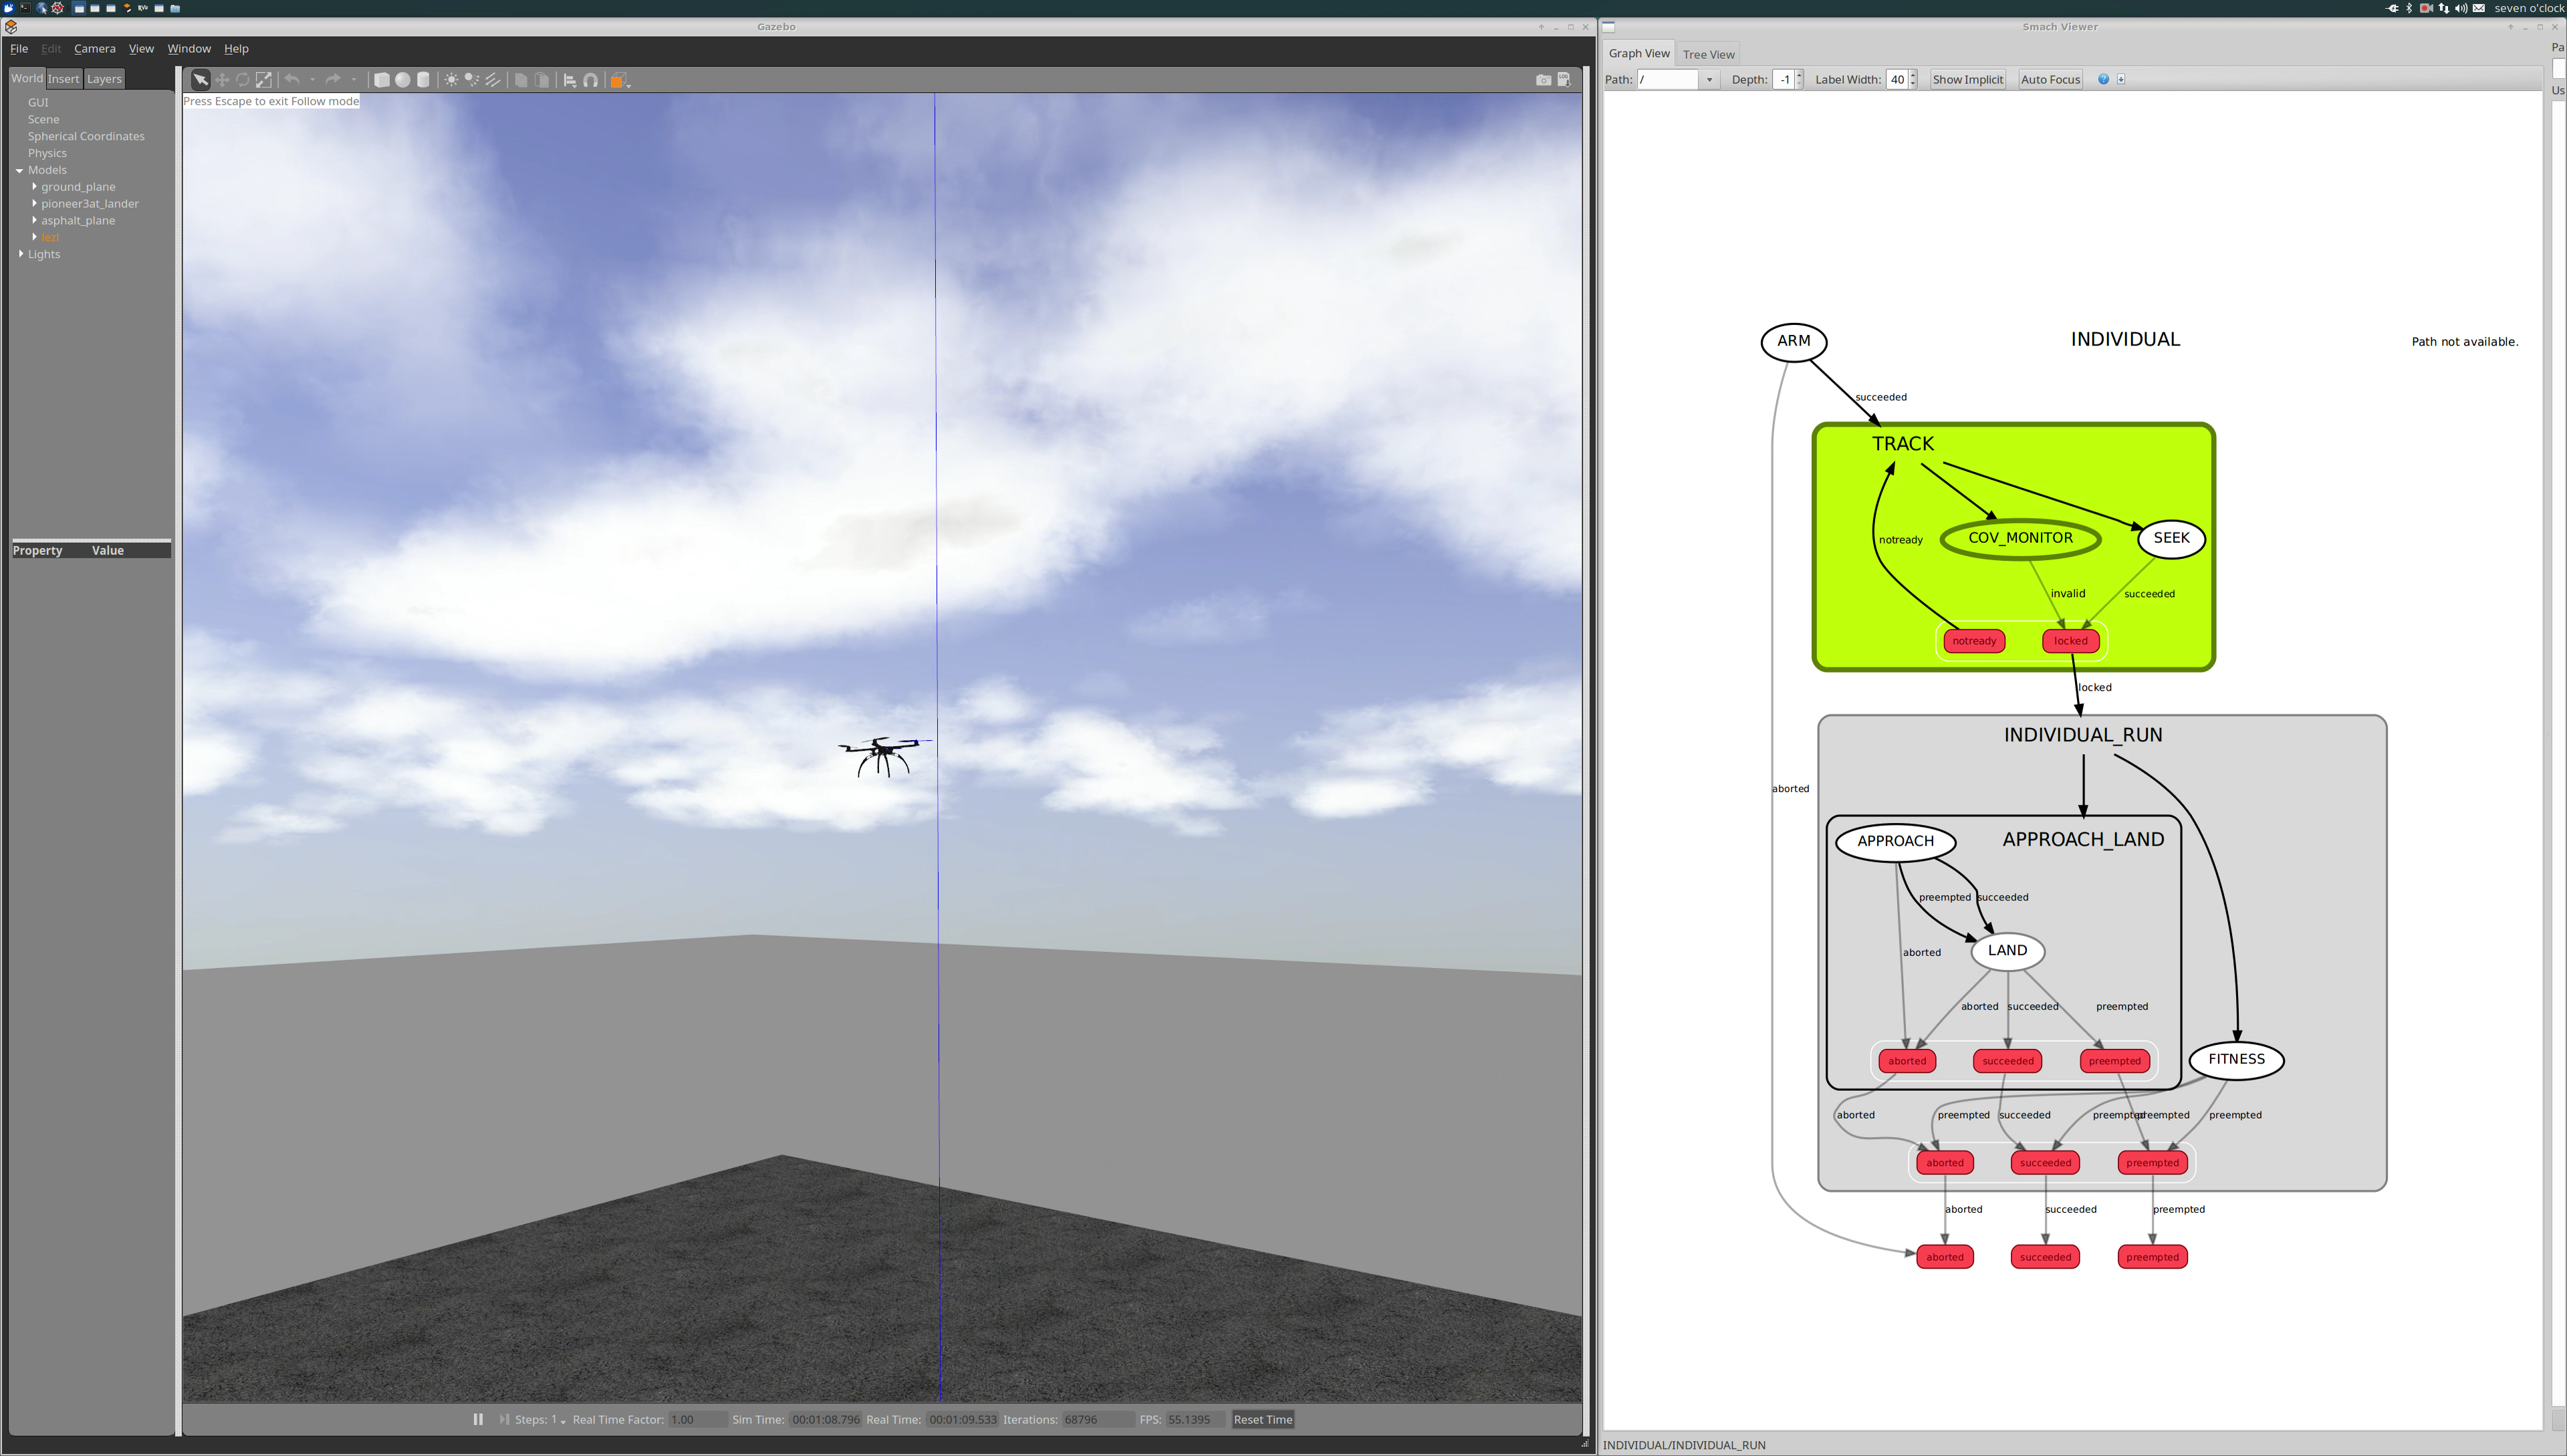
\includegraphics[width=0.8\textwidth]{images/static_captures/static-15h39m11s782}
    \caption{The ``SEEK'' substate has completed and the state machine is waiting for ``COV\_MONITOR'' to
        verify that the EKF estimate covariance is sufficiently small to signal that the vehicle has a visual
    track.}\label{f:smach_covmon}
\end{figure}

\begin{figure}
    \centering
    \includegraphics[width=0.8\textwidth]{images/static_captures/static-15h39m54s115}
    \caption{The vehicle has transitioned now to the landing approach. At this point, the FL controller is in
    command of the vehicle and all pose estimation is based on visual sensor feedback. The ``APPROACH'' state
will continue to apply FL control until either the vehicle is sufficiently close to the platform to transition
to the ``LAND'' state or loses track of the platform which will force the vehicle to abort it's
approach}\label{f:smach_approach}
\end{figure}

\begin{figure}
    \centering
    \includegraphics[width=0.8\textwidth]{images/static_captures/static-15h39m35s318}
    \caption{The vehicle has successfully approached the platform and started the landing
    sequence.}\label{f:smach_land}
\end{figure}

\begin{figure}
    \centering
    \includegraphics[width=0.8\textwidth]{images/static_captures/static-15h40m36s328}
    \caption{The vehicle is landed on the platform and motors are disarmed at mission
    success.}\label{f:smach_complete}
\end{figure}

